\section{Messungen}

\subsection{Sendeeinheit}
Die folgenden Grafiken(Abb. \ref{fig:measMiller}) zeigen das Eingangssignal(obere Kurve), das Dreieckssignal des Miller-Integrator(mittlere Kurve) und die daraus synthetisierte PWM(untere Kurve) in jeweils 2 Zeitauflösungen. Die obere Grafik ist dabei mit 2 ms/DIV und die untere Grafik mit 1ms/DIV aufgelöst. Diese Messung bestätigt damit die Simluation aus Abschnitt \ref{sec:simMiller}. Die Frequenz des wurde zu Demonstrationszwecken auf ca. 2kHz verringert um die Änderung des Tastverhältnisses des Rechtecksignals reltiv zum Eingangssignal darzustellen. Gut zu erkennen ist, dass sich die Fläche unter dem Rechtecksignal relativ zum Eingangssignal ändert und damit der Effektivwert des Rechtecksignals.(siehe Abschnitt \ref{sec:pwmTheory}).
\begin{figure}[H]
	\centering
	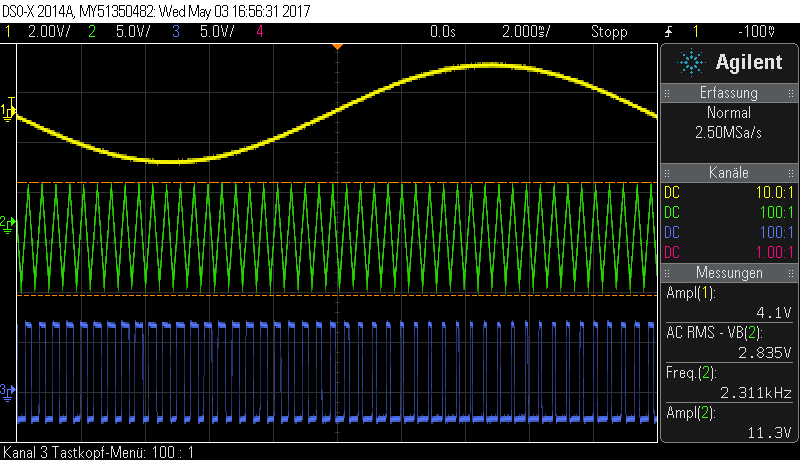
\includegraphics[scale=0.5]{gfx/osziScreens/scope_3.png}
	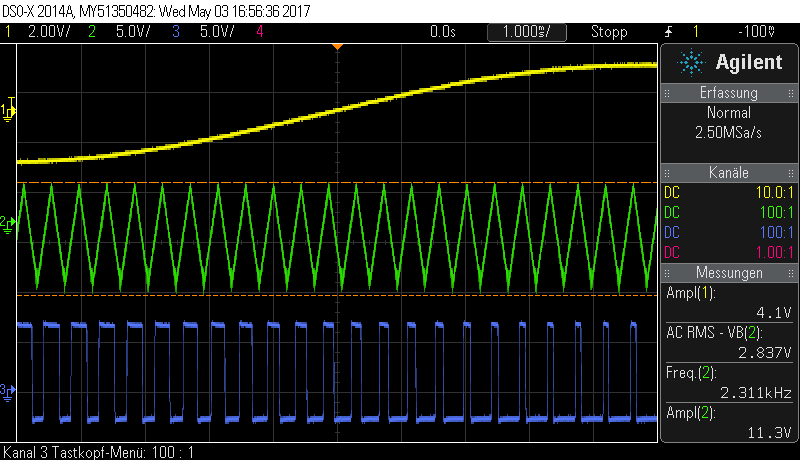
\includegraphics[scale=0.5]{gfx/osziScreens/scope_4.png}
	\caption{Eingangssignal,Dreieck und PWM}
	\label{fig:measMiller}
\end{figure}
\subsection{Empfangseinheit}
Die folgenden Messungen zeigen die Filterung des Empfangssignals in verschiedenen Filterstufen(Kurven je Grafik) und zu verschiedenen Zeitauflösung\-en(obere und untere Grafik). Die obere Kurve zeigt das empfangene Signal direkt vor dem Tiefpass. Die mittlere Kurve zeigt das Signal nach dem passiven Tiefpass(vgl. Abb. \ref{fig:design_report} $R_1,C_1$). Die untere Kurve zeigt das empfangene Signal nach dem Tiefpass und vor dem Endverstärker. Die Grafiken zeigen die Kurven jeweils bei einer Zeitauflösung von 10ms/DIV(obere Grafik) und 2ms/DIV(untere Grafik. Bei der Zeitauflösung von 2ms/DIV ist sehr gut zu erkennen, dass nach dem ersten Tiefpass, das Signal aus einem Sinus, welcher mit einem Dreieckssignal überlagert ist, besteht und nach weiterer Filterung dieses hochfrequente Dreieckssignal komplett verschwindet. Dies bestätigt den Frequenzgang aus Abbildung \ref{fig:frequencyResponse}.
\begin{figure}[H]
	\centering
	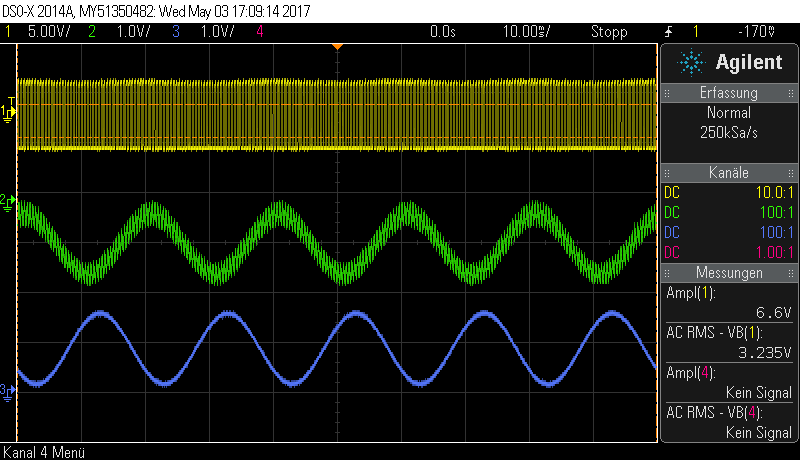
\includegraphics[scale=0.5]{gfx/osziScreens/scope_10.png}
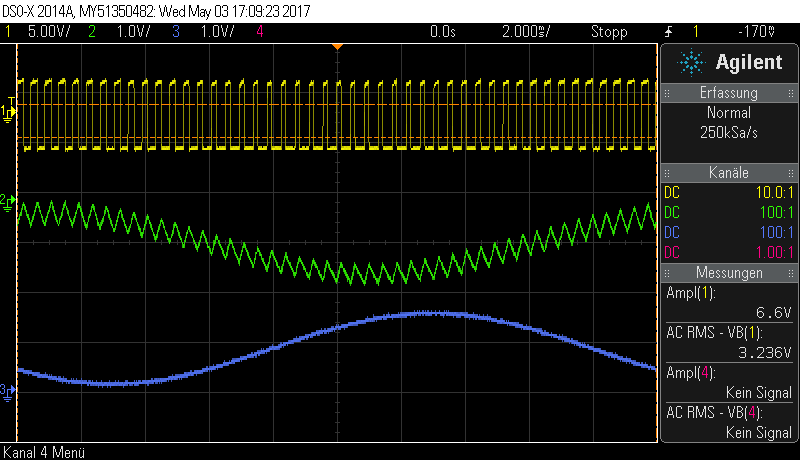
\includegraphics[scale=0.5]{gfx/osziScreens/scope_11.png}
	\caption{Emfangssignal in verschiedenen Filterstufen}
\end{figure}
\subsection{Gesamtsystem}
In dieser Messung wurde die Linearität des Gesamtsystems geprüft. Die obere Kurve zeigt das Eingangssignal vor der Sendeeinheit, die untere Kurve zeigt das Ausgangssignal nach der Empfangseinheit. Zu Testzwecken wurde die Verstärkung der Empfangseinheit, so justiert, dass bei kleiner Eingangsspannung(ca. $4V_{pp}$) an der Sendeeinheit auch selbige von der Empfangseinheit am Ausgang wiedergegeben wird. 
\begin{figure}[H]
  \centering
   \subfigure[5V Eingangsspannung]{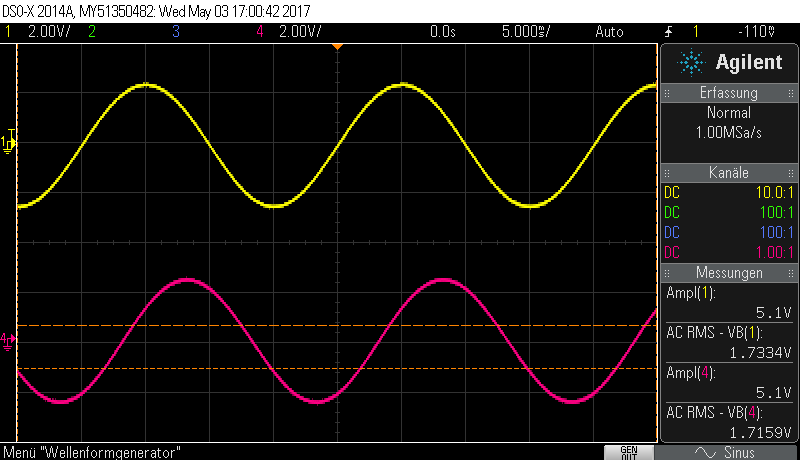
\includegraphics[scale=0.2]{gfx/osziScreens/scope_6.png}}\qquad
   \subfigure[4V Eingangsspannung]{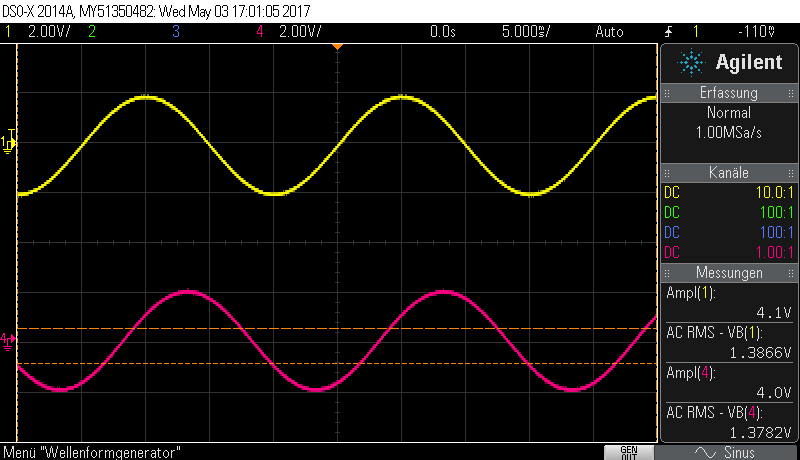
\includegraphics[scale=0.2]{gfx/osziScreens/scope_7.png}}\\
   \subfigure[3V Eingangsspannung]{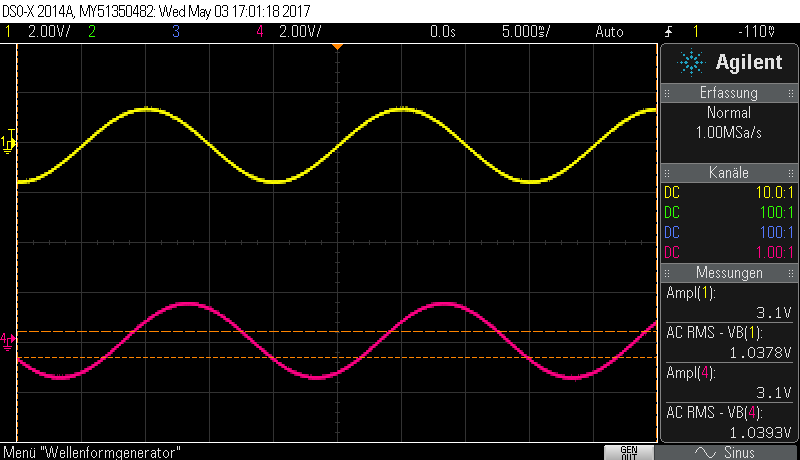
\includegraphics[scale=0.2]{gfx/osziScreens/scope_8.png}}\qquad
   \subfigure[2V Eingangsspannung]{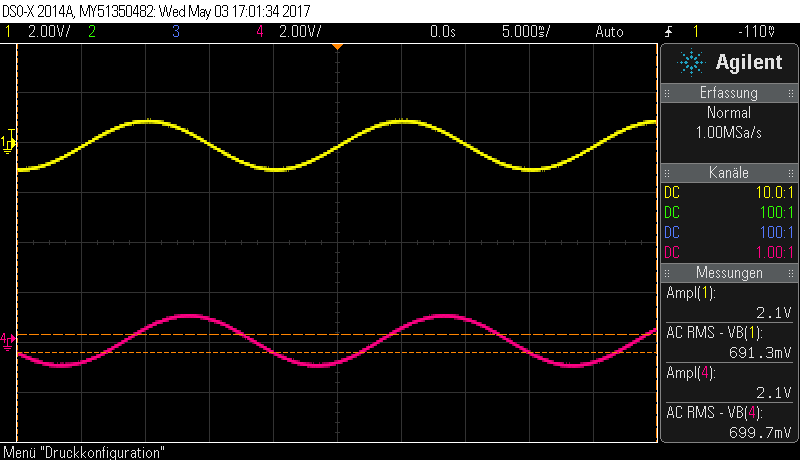
\includegraphics[scale=0.2]{gfx/osziScreens/scope_9.png}}
  \caption{Linearität des Gesamtsystems}
\end{figure}

Zur Überprüfung der Linearität wird der Quotient aus Eingangssignal und Ausgangssignal gebildet. Die folgende Tabelle(Tabelle \ref{tab:lin}) zeigt einen annährend gleichbleibenden Quotienten und somit, dass das Gesamtsystem linear ist. 
\begin{table}[H]
\centering
\begin{tabular}{clll}
\cline{1-4}
Messung & $\frac{U_{ein}}{V}$ & $\frac{U_{aus}}{V}$ &$\frac{U_{ein}}{U_{aus}}$ \\ 
\cline{1-4}
a & 5,1                                        & 5,1                                       & 1                         \\
b & 4,1                                        & 4,0                                       & 1.025                     \\
c & 3,1                                        & 3,1                                       & 1                         \\
d & 2,1                                        & 2,1                                       & 1                        
\end{tabular}
\caption{Linearitätsprüfung des Gesamtsystems}
\label{tab:lin} 
\end{table}






